\subsection{Υλοποίηση με Τεχνικές Μηχανικής Εκμάθησης}
Μια διαφορετική υλοποίηση που έχουμε να προτείνουμε είναι μια προσέγγιση με τεχνικές Μηχανικής Μάθησης. Όπως αναφέρεται και στο \cite{mldef}, η Μηχανική Μάθηση είναι υποπεδίο της επιστήμης των υπολογιστών που αναπτύχθηκε από τη μελέτη της αναγνώρισης προτύπων και της  υπολογιστικής θεωρίας μάθησης στην τεχνητή νοημοσύνη. Πιο συγκεκριμένα, κάνουμε χρήση επιβλεπόμενης μάθησης (supervised learning) κατά την οποία το υπολογιστικό πρόγραμμα δέχεται τις παραδειγματικές εισόδους καθώς και τα επιθυμητά αποτελέσματα από έναν «δάσκαλο», και ο στόχος είναι να μάθει έναν γενικό κανόνα προκειμένου να αντιστοιχίσει τις εισόδους με τα αποτελέσματα.
Πιο αναλυτικά:
\begin{itemize}
	\item \textbf{Παραδειγματικοί είσοδοι:} Αρχεία Wav των 8 KHz, 8 bit, mono των 8s εκτελεσμένα από διάφορους χρήστες από τη βάση MIR-QBSH-corpus \cite{jang-dataset}.
	\item \textbf{Χαρακτηριστικά (features):} 14 Pitch Vectors μέσω της μεθόδου Cepstral\cite{cepstral} (η επιλογή της οποίας έγινε ύστερα από σύγκριση Pitch vectors διαφορετικών και κοινών τραγουδιών) με μήκος παραθύρου 1s και μήκος επικάλυψης 0.5s. Ο λόγος είναι γιατί θεωρήσαμε, ότι το ένα δευτερόλεπτο αρκεί για να περιγράψει επαρκώς ένα σημείο του τραγουδιού.
	\item \textbf{Επιθυμητά αποτελέσματα:} Τα labels των παραπάνω τραγουδιών, δηλαδή το τίτλο του καθενός.
\end{itemize}

\begin{figure}
	\centering
	\vspace{-20pt}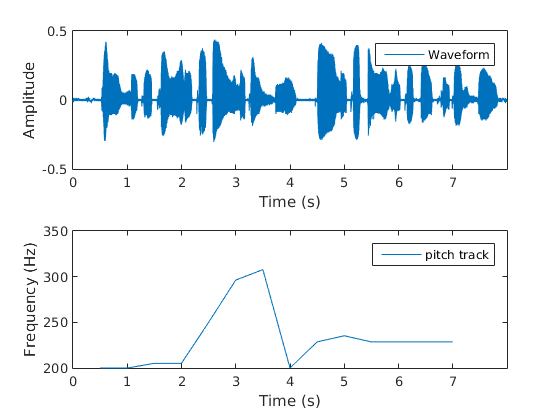
\includegraphics[height=7cm, width=\linewidth]{machine_learning/pitchvector_cepstrum}
	\vspace{-20pt}\caption{Pitch Vectors με παράθυρο 1000ms και επικάλυψη 50\%.}
	\label{fig:pvcepstrum}
\end{figure}

Σημαντικό είναι να πούμε ότι χρησιμοποιήσαμε μικρό πλήθος τραγουδιών και συγκεκριμένα 9 λόγω του μικρού μεγέθους των δειγμάτων που είχαμε και σε σχέση με αυτό των features που επιλέξαμε. Επίσης κάναμε τις εξής θεωρήσεις, οι οποίες προέκυψαν από τη βάση δεδομένων που χρησιμοποιήσαμε:
\begin{enumerate}
	\item Καθώς χρησιμοποιούμε παράθυρα των 1s με overlap \textit{50\%}, θεωρούμε ότι τα κομμάτια θα πρέπει να είναι εκτελεσμένα με καθυστέρηση το πολύ 500ms (π.χ. λόγω διαφορετικού tempo).
	\item Η εκτέλεση του κάθε τραγουδιού ξεκινάει πάντα από την αρχή.
\end{enumerate}
Στην αρχή χρησιμοποιήθηκαν μοντέλα μηχανικής εκμάθησης, τα οποία φαίνονται στην εικόνα \ref{fig:matlab_ml_alg}. Ενδεικτικά κάποια από αυτά είναι:

\begin{itemize}
	\item Δέντρα Απόφασης (Complex Trees) - Overall Accuracy \textit{55.3\%}
	\item k-Nearest Neighbors Algorithm 	- Overall Accuracy \textit{54.7\%}
	\item Cubic Support Vector Machines	- Overall Accuracy \textit{67.9\%}
\end{itemize}

\begin{figure}
	\centering
	\vspace{-20pt}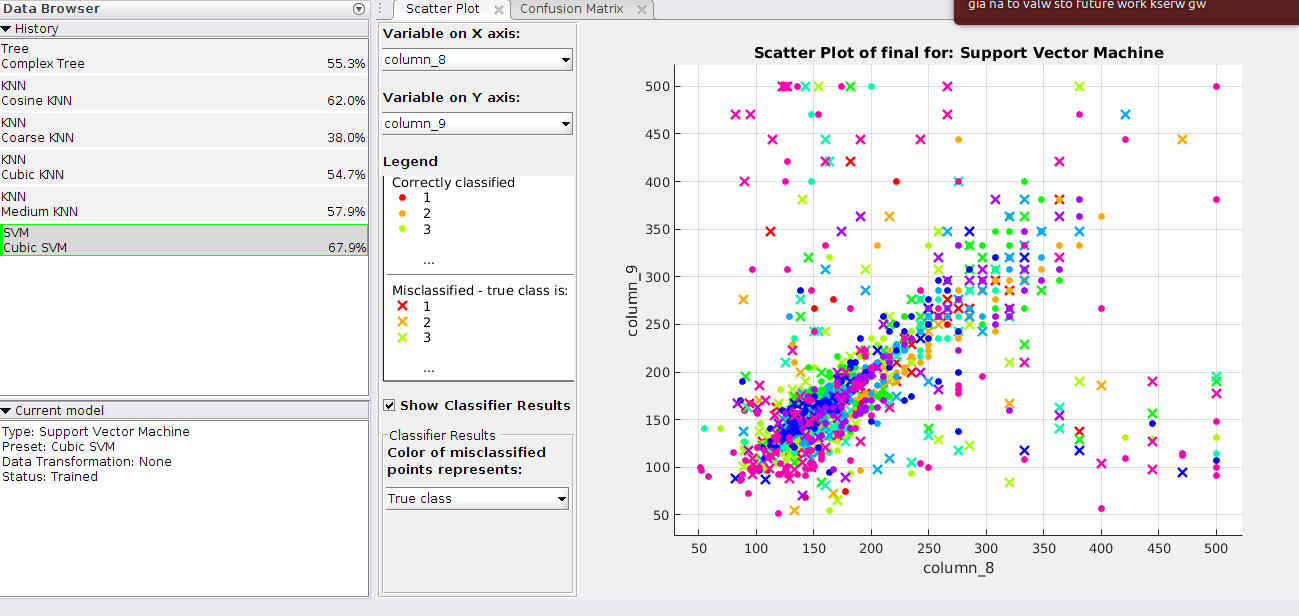
\includegraphics[height=7cm, width=\linewidth]{machine_learning/matlab_working_ml_alt}
	\vspace{-20pt}\caption{Αλγόριθμοι Μηχανικής μάθησης σε Matlab R2015a \cite{matlab} που απέτυχαν.}
	\label{fig:matlab_ml_alg}
\end{figure}

Όπως φαίνεται και από τις παραπάνω μετρικές, οι συγκεκριμένοι τρόποι μηχανικής εκμάθησης δεν μας δώσανε τα επιθυμητά αποτελέσματα. Γιαυτό το λόγο, χρησιμοποιήσαμε Νευρωνικά Δίκτυα και το πρόγραμμα Matlab R2015a \cite{matlab}. Το νευρωνικό δίκτυο είναι ένα δίκτυο από απλούς υπολογιστικούς κόμβους (νευρώνες), διασυνδεδεμένους κατάλληλα μεταξύ τους με κύριο χαρακτηριστικό την εγγενή ικανότητα μάθησης. Ως μάθηση μπορεί να οριστεί η σταδιακή βελτίωση της ικανότητας του δικτύου να επιλύει κάποιο πρόβλημα (π.χ. η σταδιακή προσέγγιση μίας συνάρτησης)\cite{neural_net}. Ύστερα από αρκετές δοκιμές καταλήξαμε σε 40 νευρώνες χωρίζοντας τα δείγματα μας σε Training set(\textit{80\%}), Validation set(\textit{10\%}) και Testing set (\textit{10\%}). Επιλέξαμε τόσο χαμηλά ποσοστά, ενώ στη βιβλιογραφία χρησιμοποιούνται συνήθως \textit{15\%}, λόγω του μικρού πλήθους δειγμάτων που είχαμε. Στην εικόνα \ref{fig:matlab-results} παρουσιάζονται τα αποτελέσματα μετά από την εκπαίδευση του νευρωνικού.

\begin{figure}[htb]
	\centering
	\begin{subfigure}{0.5\linewidth}
		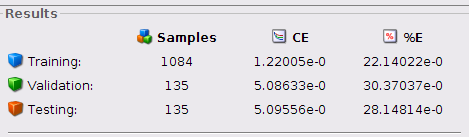
\includegraphics[width=\linewidth, keepaspectratio]{machine_learning/nn_results}
	\end{subfigure}\hfill
	\begin{subfigure}{\linewidth}
		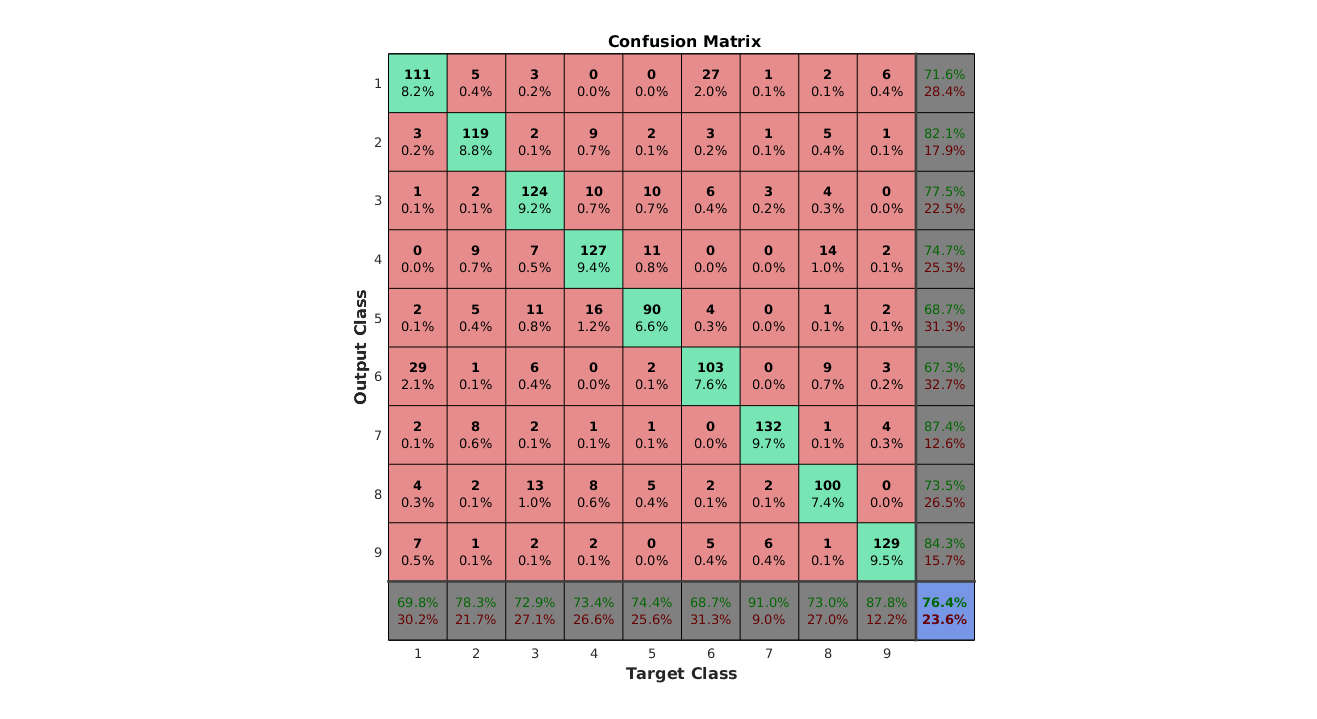
\includegraphics[width=\linewidth, keepaspectratio]{machine_learning/confusion_matrix}
	\end{subfigure}
	\caption{\textit{Cross Entropy Error/Classification Error} και \textit{Confusion Matrix} του Νευρωνικού Δικτύου.}
	\label{fig:matlab-results}
\end{figure}

Επίσης για τα πλαίσια της παρουσίασης υλοποιήθηκε ένα μικρό script το οποίο ηχογραφεί τον χρήστη για 8 δευτερόλεπτα, εξάγει τα Pitch Vectors, τα εισάγει στο νευρωνικό δίκτυο και εκτυπώνει το τελικό label, δηλαδή τον τίτλο του τραγουδιού.